

\chapter{Plano de Gerenciamento de Riscos}
  	\label{plano_de_riscos}
% 	\input{anexos/Plano_de_Gerenciamento_de_riscos}

%%%%%%%%%%%%%%%%%%%%%%% PLANO DE GERENCIAMENTO DE RISCOS

\begin{center}
 {\large Plano de gerenciamento de riscos}\\[0.2cm]
 {Bancada para Ensaios de Vibração Mecânica}\\
 \end{center}

 \section*{Histórico de Alterações}
\begin{table}[h]
\centering
\begin{tabular}{|c|c|p{6cm}|p{5cm}|}

Data & Versão & Descrição & Responsável\\
\hline
01/09/2016 & 1.0 & Criação do Plano de Gerenciamento de Riscos & Ítalo Paiva.
\\
\hline
\end{tabular}
\end{table}

\section*{Objetivo}
O objetivo desse plano é estabelecer um processo de gerenciamento de riscos do projeto e comunicar os riscos do projeto identificados.

\section*{Descrição dos processos de gerenciamento de riscos}

O Gerenciamento de Riscos possui processos definidos de seu planejamento, identificação, análise, planejamento de respostas e controle de riscos de um projeto \cite{pmbok}.
Para o plano de gerenciamento de riscos do projeto, os processos adotados serão os seguintes:

\begin{itemize}
  \item \textbf{Identificar os riscos} - processos de identificação de riscos que podem afetar o desenvolvimento do projeto.
  \item \textbf{Realizar a análise qualitativa dos riscos} - processo de priorização dos riscos identificados para avaliação de sua probabilidade de ocorrência e análise de seu impacto.
  \item \textbf{Planejar as respostas aos riscos} - processo que determina respostas às ocorrências de riscos para diminuir seu impacto e para reduzir ameaças às fases de desenvolvimento do projeto.
  \item \textbf{Controlar os riscos} - processo que acompanha e monitora os riscos identificados, identifica novos riscos e avalia a eficácia do processo de gerenciamento de riscos em todas as fases de desenvolvimento do projeto.
\end{itemize}

\section*{EAR – Estrutura Analítica de Riscos para identificação dos riscos}

  O Project Management Institute (PMI), criador do PMBoK, elaborou uma Estrutura Analítica de Riscos genérica para identificação dos riscos de um projeto a partir de categorias e subcategorias.
  \begin{figure}[h]
    \label{fig:ear_padrao}
    \begin{center}
    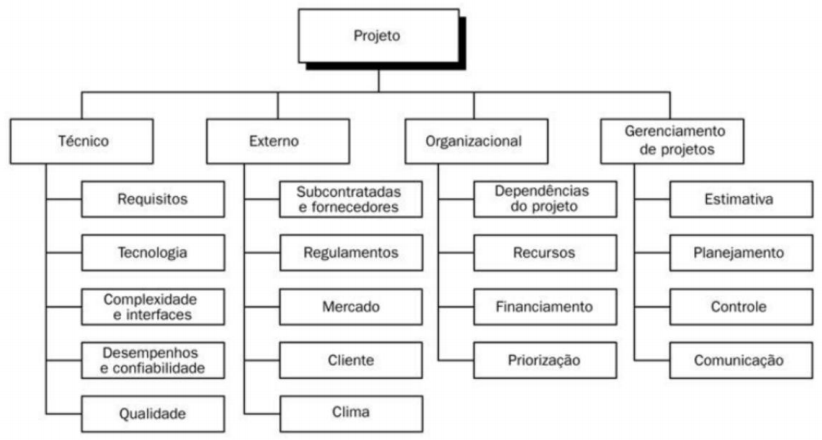
\includegraphics[scale=0.65]{figuras/ear_padrao.png}
    \end{center}
    \caption{Classificação dos riscos na EAR segundo o PMI}
  \end{figure}

As categorias e subcategorias foram analisadas em relação ao projeto e o resultado dessa análise está ilustrado nas Figuras \ref{fig:riscos_tecnicos}, \ref{fig:riscos_externos} e \ref{fig:riscos_gerenciamento}.

  \begin{figure}[h]
    \begin{center}
    \label{fig:riscos_tecnicos}
    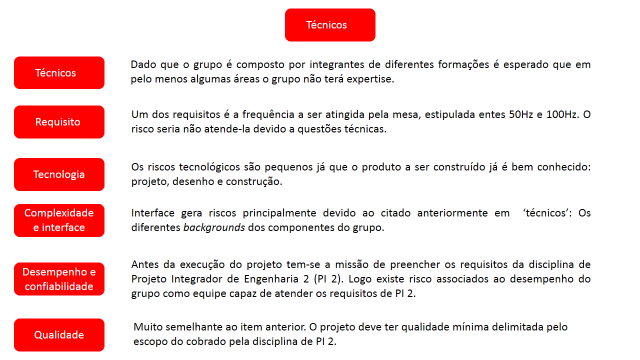
\includegraphics[scale=0.65]{figuras/riscos_tecnicos.png}
    \end{center}
    \caption{Análise em relação aos riscos técnicos}
  \end{figure}

  \begin{figure}[h]
    \begin{center}
    \label{fig:riscos_externos}
    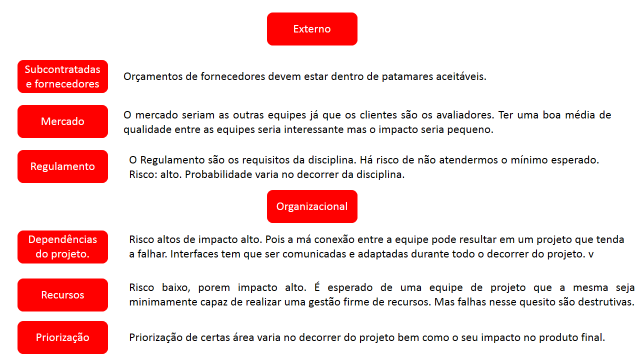
\includegraphics[scale=0.65]{figuras/riscos_externos_organizacional.png}
    \end{center}
    \caption{Análise em relação aos riscos externos e organizacionais}
  \end{figure}

  \begin{figure}[ht]
    \begin{center}
    \label{fig:riscos_gerenciamento}
    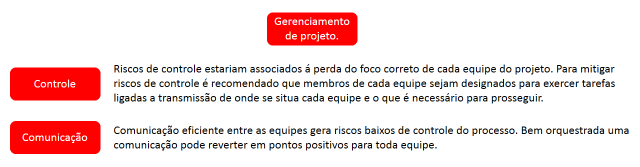
\includegraphics[scale=0.65]{figuras/riscos_gerenciamento.png}
    \end{center}
    \caption{Análise em relação aos riscos de gerenciamento}
  \end{figure}

\vfill
\pagebreak

\section*{Qualificação dos riscos}
Os riscos identificados serão qualificados na sua probabilidade de ocorrência e impacto nos resultados, conforme as Tabelas \ref{probabilidade_riscos} e \ref{impacto_riscos} ilustram.

\begin{table}[h]
\centering
\caption{Probabilidade dos riscos}
\label{probabilidade_riscos}
\begin{tabular}{|l|l|}
\hline
\multicolumn{1}{|c|}{\textbf{Nível}} & \multicolumn{1}{c|}{\textbf{Descrição}} \\ \hline
Baixo                                & Muito improvável (0\% - 30\%)       \\ \hline
Médio                                & Pouco provável (31\% - 60\%)            \\ \hline
Alto                                 & Provável (61\% - 90\%)                  \\ \hline
\end{tabular}
\end{table}


\begin{table}[h]
\centering
\caption{Impacto dos riscos}
\label{impacto_riscos}
\begin{tabular}{|l|l|}
\hline
\multicolumn{1}{|c|}{\textbf{Nível}} & \multicolumn{1}{c|}{\textbf{Descrição}} \\ \hline
Baixo & Tem pouco prejuízo ao desenvolvimento do projeto \\ \hline
Médio & Prejudica o desenvolvimento do projeto, mas de rápida resiliência \\ \hline
Alto & Tem muito prejuízo ao desenvolvimento do projeto \\ \hline
\end{tabular}
\end{table}

\subsection*{Prioridade dos riscos}

A prioridade dos riscos é dada pelo produto cartesiano da probabilidade e do impacto, conforme a Tabela \ref{prioridade_riscos}.

\begin{table}[h]
\centering
\caption{Classificação da Prioridade}
\label{prioridade_riscos}
\begin{tabular}{|
>{\columncolor[HTML]{9B9B9B}}c |
>{\columncolor[HTML]{34FF34}}c |c|
>{\columncolor[HTML]{FE0000}}c |}
\hline
\textbf{Provável} & \cellcolor[HTML]{FCFF2F}\textbf{Risco médio} & \cellcolor[HTML]{FE0000}\textbf{Risco alto} & \textbf{Risco extremo} \\ \hline
\textbf{Pouco provável} & \textbf{Risco baixo} & \cellcolor[HTML]{FCFF2F}\textbf{Risco médio} & \textbf{Risco alto} \\ \hline
\textbf{Muito improvável} & \textbf{Risco insignificante} & \cellcolor[HTML]{34FF34}\textbf{Risco baixo} & \cellcolor[HTML]{FCFF2F}\textbf{Risco médio} \\ \hline
\cellcolor[HTML]{656565}\textbf{Probabilidade/Impacto} & \cellcolor[HTML]{9B9B9B}\textbf{Baixo} & \cellcolor[HTML]{9B9B9B}\textbf{Médio} & \cellcolor[HTML]{9B9B9B}\textbf{Alto} \\ \hline
\end{tabular}
\end{table}

\subsection*{Riscos Identificados - Ponto de Controle 1}

Os riscos identificados para o projeto estão listados na Tabela \ref{riscos_projeto}.

\begin{table}[h]
\centering
\caption{Riscos Identificados para o Projeto}
\label{riscos_projeto}
\begin{tabular}{|l|l|l|c|}
\hline
\multicolumn{1}{|c|}{\textbf{Risco}} & \multicolumn{1}{c|}{\textbf{Probabilidade}} & \multicolumn{1}{c|}{\textbf{Impacto}} & \textbf{Prioridade} \\ \hline
Algum membro abandonar a equipe & Baixa & Alto & \cellcolor[HTML]{FCFF2F}\textbf{Média} \\ \hline
Não houver financiamento suficiente. & Média & Alto & \cellcolor[HTML]{FE0000}\textbf{Alta} \\ \hline
\begin{tabular}[c]{@{}l@{}}Não conseguir os materiais\\  necessários para o produto por\\  tempo e localização.\end{tabular} & Baixa & Alto & \cellcolor[HTML]{FCFF2F}\textbf{Média} \\ \hline
Houver atrasos entre as equipes. & Média & Alto & \cellcolor[HTML]{FE0000}\textbf{Alta} \\ \hline
\begin{tabular}[c]{@{}l@{}}Os horários do galpão não serem\\  suficientes ou aptos.\end{tabular} & Alta & Médio & \cellcolor[HTML]{FE0000}\textbf{Alta} \\ \hline
\begin{tabular}[c]{@{}l@{}}Requisito entre as equipes serem\\ modificados no decorrer do processo.\end{tabular} & Média & Alto & \cellcolor[HTML]{FE0000}\textbf{Alta} \\ \hline
Greve & Baixa & Baixo & \cellcolor[HTML]{34FF34}\textbf{Baixa} \\ \hline
\end{tabular}
\end{table}

\subsubsection*{Ações de resposta aos riscos}

As ações definidas para reagir aos riscos identificados se encontram na Tabela \ref{acoes_riscos}.

\begin{table}[h]
\centering
\caption{Ações de contingência aos riscos}
\label{acoes_riscos}
\begin{tabular}{|c|c|}
\hline
\textbf{Risco} & \textbf{Ação de contingência} \\ \hline
Algum membro abandonar a equipe & \begin{tabular}[c]{@{}c@{}}Redistribuição de tarefas\\ 			e membros dentro da equipe\end{tabular} \\ \hline
Não houver financiamento suficiente & \begin{tabular}[c]{@{}c@{}}Modificação de parâmetros pontuais\\  com o objetivo de reduzir os custos\end{tabular} \\ \hline
\begin{tabular}[c]{@{}c@{}}Não conseguir os materiais\\  necessários para o produto por\\  tempo e localização\end{tabular} & \begin{tabular}[c]{@{}c@{}}Modificação de parâmetros pontuais com\\ o objetivo de adaptar o projeto a essa\\ 			situação, caso não encontre novos fornecedores\end{tabular} \\ \hline
Houver atrasos entre as equipes & \begin{tabular}[c]{@{}c@{}}Inicialmente,  comunicação\\ 			perante a equipe e busca de soluções internamente\\ 			\\ 			Em ultima instância,\\ 			comunicação aos professores da disciplina\end{tabular} \\ \hline
\begin{tabular}[c]{@{}c@{}}Os horários do galpão não serem\\  suficientes ou aptos\end{tabular} & \begin{tabular}[c]{@{}c@{}}Atividade será reposicionada para outro\\  local, na medida do possível\\  (local a definir com a equipe)\end{tabular} \\ \hline
\begin{tabular}[c]{@{}c@{}}Requisito entre as equipes serem\\ modificados no decorrer do processo\end{tabular} & \begin{tabular}[c]{@{}c@{}}Modificação de parâmetros pontuais\\ com o objetivo de adequar requisitos\end{tabular} \\ \hline
Greve & \begin{tabular}[c]{@{}c@{}}Os trabalhos continuarão e serão  readaptados\\  para os novos horários\end{tabular} \\ \hline
\end{tabular}
\end{table}

\subsection*{Sistema de Controle de mudanças de riscos}

Para controlar riscos e tentar de alguma forma amenizar percalços que possam atingir o projeto futuramente, o controle de riscos assume os problemas que possam surgir no decorrer do trabalho, de maneira que, caso aconteça algum risco não planejado, a resposta lógica da equipe será retornar ao documento de Gerenciamento de Risco, mensurar e analisar tal problema, assim como todos os outros, para que se possa tomar a medida mais adequada a situação.

\subsection*{Outros assuntos relacionados ao gerenciamento de riscos do projeto não previstos nesse plano}

Assuntos relacionados ao Gerenciamento de Riscos do Projeto que não foram previstos, caso aconteçam e mostrem relevância para o projeto, devem ser atualizados nesse documento, de maneira que este ande sempre alinhado com o projeto.

\section*{Riscos Identificados - Ponto de Controle 2}

Os riscos identificados para o projeto estão listados na Tabela foram divididos por cada frente do projeto

\subsection*{Riscos Gerais Identificados}

\begin{table}[H]
    \begin{tabular}{|p{7cm}|p{7cm}|}
        \hline
        \textbf{Risco} & \textbf{Ação de contigência} \\ \hline
         &  \\ \hline
         & \\ \hline
         & \\ \hline
         & \\ \hline
    \end{tabular}
    \caption{Tabela de Riscos Identificados da Frente de Mecânica - Fonte: Autores}
    \label{tab:tabela_riscos_mecanica}
\end{table}

\subsection*{Riscos Identificados - Frente Mecânica}

\begin{table}[H]
    \begin{tabular}{|p{7cm}|p{7cm}|}
        \hline
        \textbf{Risco} & \textbf{Ação de contigência} \\ \hline
        Alinhamento inadequado do contato entre tampo e estrutura. & Talhar um dos copinhos do tampo e fazer o realocamento do copinho \\ \hline
        Alinhamento inadequado dos mancais (podendo causar desalinhamento das polias). & Talhar o mancal, colocar uma chapa para gabarito no mancal e fazer a realocação \\ \hline
        Incompatibilidade das análises com as constantes consideradas com relação ao modelo real. & Redefinir os parametros de análise e repetir até acerta o valor \\ \hline
        Uso do galpão comprometido (Devido à greve dos técnicos). & Realocar a estrutura para outro lugar \\ \hline
    \end{tabular}
    \caption{Tabela de Riscos Identificados da Frente de Mecânica - Fonte: Autores}
    \label{tab:tabela_riscos_mecanica}
\end{table}

\subsection*{Riscos Identificados - Frente Eletromecânica}

\begin{table}[H]
    \begin{tabular}{|p{7cm}|p{7cm}|}
        \hline
        \textbf{Risco} & \textbf{Ação de contigência} \\ \hline
        Descargas elétricas que podem danificar o funcionamento do inversor e do motor. & O sistema de segurança foi modelado para suportar a maior parte das ocorrências conhecidas, no entanto ocorrências extraordinárias causarão de qualquer forma danos ao sistema \\ \hline
        Intervenção indevida do usuário no sistema de distribuição de potência & Foram tomados cuidados para que os terminais do sistema fossem isolados com terminais pré-isolados e luvas termoretráteis \\ \hline
        Ausência de monitoramento de corrente de falta (aterramento). & A solução seria invíavel. \\ \hline
    \end{tabular}
    \caption{Tabela de Riscos Identificados da Frente de Eletromecânica - Fonte: Autores}
    \label{tab:tabela_riscos_eletromecanica}
\end{table}

\subsection*{Riscos Identificados - Frente Eletroeletrônica}

\begin{table}[H]
    \begin{tabular}{|p{7cm}|p{7cm}|}
        \hline
        \textbf{Risco} & \textbf{Ação de contigência} \\ \hline
        Taxa de leitura de sensores abaixo da taxa de nyquist quando escalado & Trabalhar as frequencias mais baixas, ou diminuir a quantidade de sensores \\ \hline
        Estabilidade das fontes de tensão (Forte depêndencia das fontes de tensão que vierem do inversos) & Utilizar elementos de proteção na placa \\ \hline
        Aliasing no sinal de aceleração da mesa. & Fazer uma filtragem digital passa baixas no sinal \\ \hline
    \end{tabular}
    \caption{Tabela de Riscos Identificados da Frente de Eletroeletrônica - Fonte: Autores}
    \label{tab:tabela_riscos_eletroeletronica}
\end{table}

\subsection*{Riscos Identificados - Frente Interface/Processamento}

\begin{table}[H]
    \begin{tabular}{|p{7cm}|p{7cm}|}
        \hline
        \textbf{Risco} & \textbf{Ação de contigência} \\ \hline
        Massa de dados coletadas pelos sensores sendo fornecidas à uma taxa superior à capacidade de processamento do hardware & Efetuar troca do hardware disponível para atuar como servidor REST (Passar à utilizar um microcomputador ao invés de uma Raspberry PI) \\ \hline
        Atrasos existentes na rede para transmissão de pacotes de informações & Utilizar conexão de rede cabeada para evitar agressões à transmissão oriundas do meio e verificar dimensionamento da rede para não haver sobrecarga no roteador, evitando perda de pacotes. \\ \hline
        Integridade dos dados comprometida & Implementar mecanismos de checagem de integridade de dados (checksum) \\ \hline
    \end{tabular}
    \caption{Tabela de Riscos Identificados da Frente de Interface/Processamento - Fonte: Autores}
    \label{tab:tabela_riscos_interface_processamento}
\end{table}

%%%%%%%%%%%%%%%%%%%%%%% FIM PLANO DE GERENCIAMENTO DE RISCOS